\documentclass[dvipsnames,svgnames,x11names,margin=8pt]{standalone}
\usepackage{tikz}
\usetikzlibrary{decorations.text}

\begin{document}
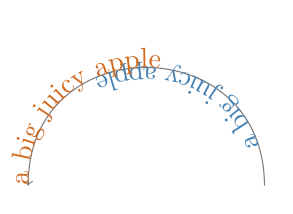
\begin{tikzpicture}

\path [draw,gray, ->] 
[postaction={
    decoration={text along path,
        text={a big juicy apple}, 
        text color=SteelBlue,
        % left indent=5mm | right indent=5mm
        text align={left indent=5mm},
        }, 
    decorate
    }
]
[postaction={
    decoration={text along path,
        text={a big juicy apple}, 
        text color=Chocolate,
        % align=left | center | right
        % text align=fit to path | fit to path stretching spaces
        text align={align=left},
        reverse path
        }, 
    decorate
    }
]
(3,0) .. controls (3,2) and (0,2) .. (0,0);

\end{tikzpicture}


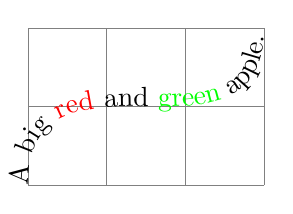
\begin{tikzpicture}
\draw [help lines] grid (3,2);
\path [decorate, 
    decoration={text along path,
        text format delimiters={[}{]},
        text={A big [\color{red}]red[] and [\color{green}]green[] apple.}
    }
]
(0,0) .. controls (0,2) and (3,0) .. (3,2);
\end{tikzpicture}

\end{document}